This is an example of a chapter\dots

\section{Section 1.1}
\subsection{Subesction 1.1.1}
Write something here...

\section{Math equations examples}

\begin{numcases}
  \displaystyle \min\,\sum_{e\in E}c_ex_e\\
  \displaystyle \sum_{e\in\delta(h)} x_e = 2 \quad \forall \ h\in V\label{HamiltCyc}
  \\
  \displaystyle \sum_{e\in\delta(S)} x_e\leq |S|-1 \quad \forall \ S\subset V : v_1 \in S\label{SEC}
  \\
  \displaystyle 0\leq x_e\leq1 \quad\mbox{integer} \quad \forall \ e\in E
\end{numcases}\\
Constraints \ref{HamiltCyc} impose that every node of the graph must be touched by exactly two edges of the cycle. This group of contraints alone isn't enough to guarantee to find a valid Hamiltonian Cycle: we could find lots of isolated cycles.

\newpage

\section{Pseudocode examples}

\begin{algorithm}
    \caption{Greedy algorithm for the TSP}
    \hspace*{\algorithmicindent} \textbf{Input} Starting node $s\in V$, Set of nodes $V$\\
    \hspace*{\algorithmicindent} \textbf{Output} List of $n\coloneq|V|$ nodes forming an Hamiltonian Cycle, Cost of the cycle
    \begin{algorithmic}

        \State $\mbox{cycle} \gets [s]$
        \State $\mbox{cost} \gets 0$
        
        \For{$i=0 \mbox{ to } n-2$}
            \State $\mbox{next} \gets \mbox{argmin}_{v}{\{c_{cycle[i], v}\;|\;v\not\in \mbox{cycle}\}}$
            \State $\mbox{cost}\gets\mbox{cost}+c_{cycle[i], next}$
            \State $\mbox{cycle}[i+1]\gets\mbox{next}$
        \EndFor
        \State $\mbox{cost}\gets\mbox{cost}+c_{cycle[n-1],s}$\\\\

        \Return cycle, cost
    \end{algorithmic}
\end{algorithm}

\section{Graphs examples}

\begin {center}
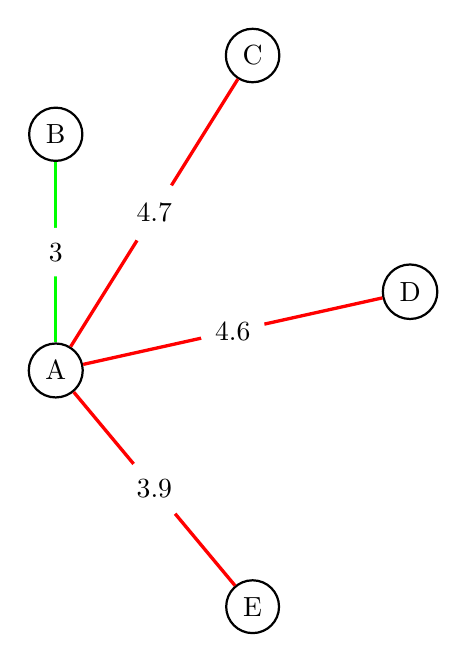
\begin{tikzpicture}
\begin{scope}[every node/.style={circle,thick,draw}]
    \node (A) at (0,0) {A};
    \node (B) at (0,3) {B};
    \node (C) at (2.5,4) {C};
    \node (D) at (4.5,1) {D};
    \node (E) at (2.5,-3) {E};
\end{scope}

\begin{scope}[every node/.style={fill=white,circle},
              every edge/.style={draw=red,very thick}]
    \path [-] (A) edge[draw=green] node {$3$} (B);
    \path [-] (A) edge node {$4.7$} (C);
    \path [-] (A) edge node {$4.6$} (D);
    \path [-] (A) edge node {$3.9$} (E);
    %\path [->] (B) edge[bend right=60] node {$1$} (E); 
\end{scope}
\end{tikzpicture}
\end{center}

\subsection{Example of citations}

This is a citation to Imai \cite{Imai15}.\\

This is a citation to Rankooh \cite{Rankooh22}.\\

This is a citation to Johnson \cite{Johnson75}.
